\paragraph{Опыт Девисона-Джермера (монокристалл)}
\begin{wrapfigure}{r}{0.5\linewidth}
	\centering
	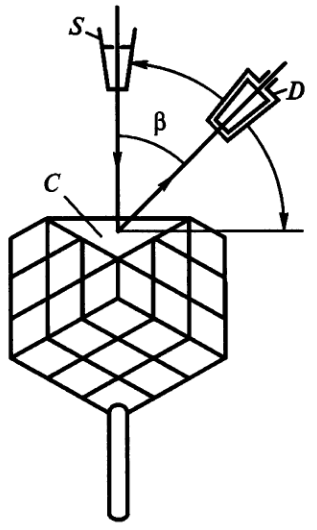
\includegraphics[width=0.5\linewidth]{img/oral-05/devison-djermer}
	\caption{Схема опыта Девисона-Джермера}
	\label{fig:devison-djermer}
\end{wrapfigure}
Электроны от электронной пушки $S$, прошедшие ускоряющую разность потенциалов $U$, падали нормально на сошлифованную поверхность кристалла никеля $C$. С помощью детектора $D$ исследовалось число электронов, отраженных от кристалла под углом $\beta$ при различных значениях $U$. Напомним, что разным значениям $U$ соответствуют разные дебройлевские длины волн электронов.

В опытах наблюдалось максимальное отражение электронов при ускоряющей разности потенциалов $U=54$ В (см. Рис \ref{fig:devison-djermer-electron-difraction-dynamics}), что соответсвует дебройлевской длине волны
\begin{equation*}
	\lambda_{\text{Б}}=\frac{2\pi\hbar}{\sqrt{2m_eeU}}=0.167 \text{нм}
\end{equation*}

Из условия Брэгга-Вульфа 
\begin{equation*}
	2d\sin\theta=n\lambda_{\text{Б}}
\end{equation*}
для постоянной решетки никеля $d=2.15\cdot10^{-10}$ определяется, <<теоретическая>> дебройлевская длина волны, она равняется $\lambda_{\text{Б}}=0.165$ нм, что отлично соотносится с результатами опыта и служит подтверждением гипотезы де Бройля.

\begin{figure}[H]
	\centering
	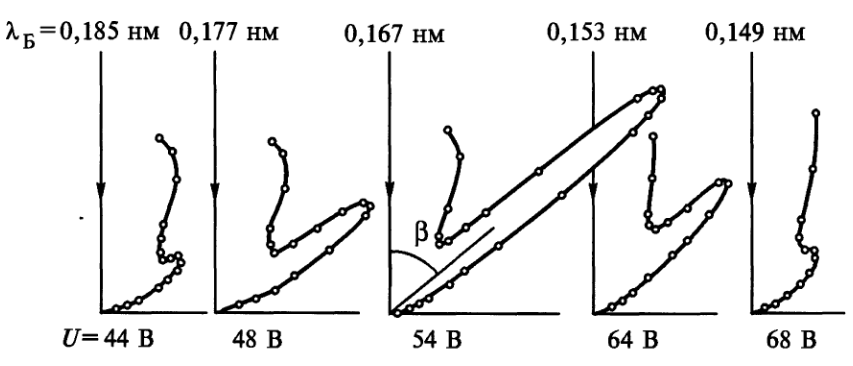
\includegraphics[width=0.8\linewidth]{img/oral-05/devison-djermer-electron-difraction-dynamics}
	\caption{Динамика дифракционного отражения электронов при изменении ускоряющей разности потенциалов $U$}
	\label{fig:devison-djermer-electron-difraction-dynamics}
\end{figure}

Была также измерена интенсивность дифрагирующих электронов в зависимости от ускоряющей разности потенциалов $U$ (см. Рис \ref{fig:devison-djermer-intensivnost-u}). Максимумы остоят друг от друга на равном по шкале $\sqrt{U}$ расстоянии, что подтверждается теорией.
\begin{equation*}
	\lambda_{\text{Б}}=\frac{2\pi\hbar}{\sqrt{2m_eE_k}}=\frac{2\pi\hbar}{\sqrt{2m_eeU}}\implies2d\sin\theta=n\frac{2\pi\hbar}{\sqrt{2m_eeU_n}},
\end{equation*}
где $U_n$ --- ускоряющая разность потенциалов, соответствующая $n$-му порядку отражения.

Таким образом связь между $U_n$ и $n$ имеет вид
\begin{equation*}
	\sqrt{U_n}=Cn,\,\text{где}\: C=\frac{\pi\hbar}{d\sin\theta\sqrt{2em_e}}=\mathrm{const}
\end{equation*}

\begin{figure}[H]
	\centering
	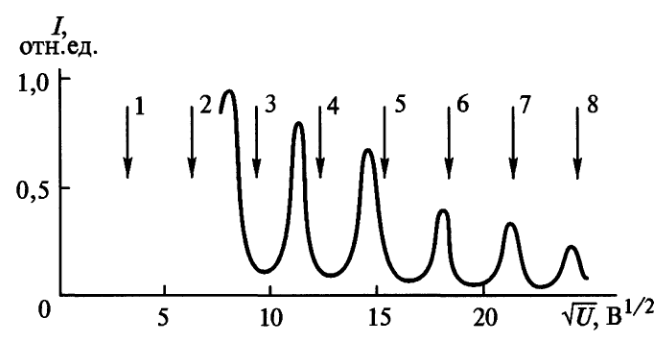
\includegraphics[width=0.5\linewidth]{img/oral-05/devison-djermer-intensivnost-u}
	\caption{Зависимость интенсивности $I$ пучка электронов, дифрагирующего на монокристалле никеля, от ускоряющего напряжения $U$ при постоянном значении угла $\theta$}
	\label{fig:devison-djermer-intensivnost-u}
\end{figure}
Различие теории и эксперимента в этом опыте заключалось в том, что положения наблюдаемых дифракционных максимумов не совпадали с положениями максимумов, определяемых из условия Брэгга — Вульфа (вертикальные стрелки на Рис. \ref{fig:devison-djermer-intensivnost-u}). Особенно заметным это различие было для небольших значений $n$, т. е. для небольшой ускоряющей разности потенциалов $U_n$. Причина такого расхождения теории и эксперимента состоит в том, что условие Брэгга — Вульфа не учитывает преломление электронных волн в металле. 
Использование условия с поправкой на преломление внутри кристалла:
\begin{equation*}
	2d\sqrt{n_e^2-\cos^2\theta}=n\lambda_{\text{Б}}
\end{equation*}
полностью устраняет это расхождение.

\paragraph{Опыты Томсона и Тартаковского (поликристалл)}
В результате наблюдале концентрические кольца, которые хорошо описывались условиями Брэгга-Вульфа
\begin{equation*}
	2d\sin\theta=n\lambda_{\text{Б}},\: R=L\tg2\theta
\end{equation*}
\begin{multicols}{2}
	\begin{figure}[H]
		\centering
		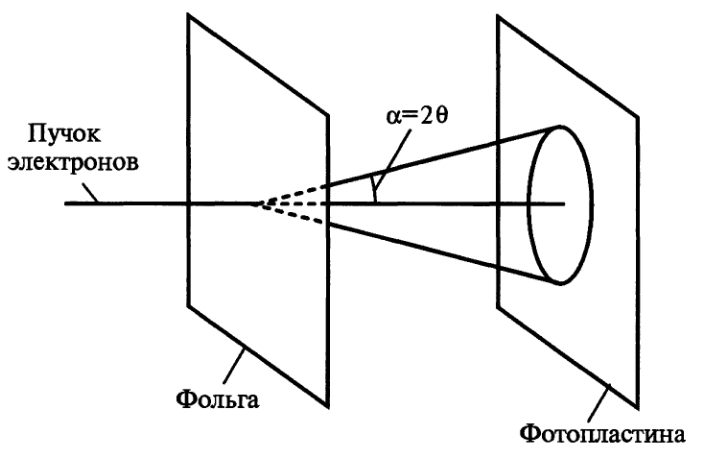
\includegraphics[width=\linewidth]{img/oral-05/tomson-tartakovsky}
		\caption{Дифракция электронов в поликристаллической фольге}
		\label{fig:tomson-tartakovsky}
	\end{figure}
	\begin{figure}[H]
		\centering
		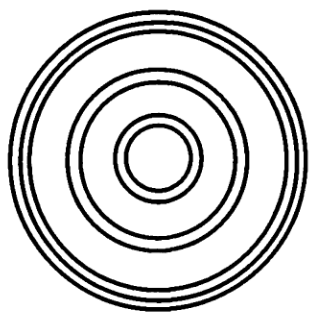
\includegraphics[width=0.64\linewidth]{img/oral-05/tomson-tartakovsky-results}
		\caption{Результаты дифракционных опытов с электронами на поликристалле серебра}
		\label{fig:tomson-tartakovsky-results}
	\end{figure}
\end{multicols}

Добавление магнитного поля между фольгой и экраном позволило подтвердить, что происходит дифракция именно электронов.

\paragraph{Опыт Фабриканта (одиночные электроны)}
В этих опытах промежуток времени между двумя последовательными прохождениями электронов через кристалл в 30 000 раз превышал время, затрачиваемое одним электроном на прохождение всего прибора. Таким образом, электроны дифрагировали в кристалле поодиночке, поэтому возникновение дифракционной картины как результата взаимодействия электронов друг с другом полностью исключалось.

Качественный вид распределения дифрагировавших электронов по фотопластинке приведен на Рис. \ref{fig:fabrikant-results}. При небольшой длительности эксперимента точки на фотопластинке, отвечающие попаданию электронов, распределены совершенно случайным образом (Рис. \ref{fig:fabrikant-results}, а). 

Однако при достаточной длительности эксперимента распределение точек приобретает характерный для дифракции на поликристалле вид концентрических колец (Рис. \ref{fig:fabrikant-results}, б). Таким образом было доказано, что волновые свойства присущи отдельному электрону.
\begin{figure}[H]
	\centering
	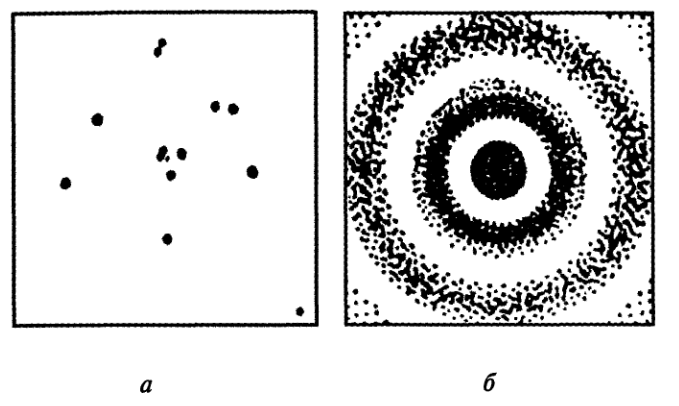
\includegraphics[width=0.45\linewidth]{img/oral-05/fabrikant-results}
	\caption{Распределение дифрагирующих электронов по фотопластинке \\ a --- при небольшой длительности эксперимента; б --- в случае длительного эксперимента;}
	\label{fig:fabrikant-results}
\end{figure}

